\chapter{Wave Motion}

The world is full of waves, with \textit{mechanical} and \textit{electromagnetic}
waves being the two main types. 
\begin{itemize}
    \item \textbf{Mechanical waves} requires that some physical medium being disturbed.
        For example, the water in a pond is disturbed when you throw a rock into it.
    \item \textbf{Electromagnetic waves} does not require a medium. For example, light can
        travel through empty space without a medium. For now, we will focus on mechanical waves.
\end{itemize}

For now, we will only focus on mechanical waves. Consider again the rock being dropped onto water.
The disturbed water molecules gains kinetic energy from the rock, and it can be transfer to another
object floating on water, causing it to move. Notice that the energy is transferred over distance,
but not matter. Also notice that the molecules of the disturbed water resembles periodic motion of
a vibrating pendulum.

\section{Propogation of a Disturbance}

All mechanical waves require the following
\begin{enumerate}
    \item a source of disturbance
    \item a medium with elements that can be disturbed
    \item a physical mechanism that allows each element to influence each other
\end{enumerate}

A \textbf{pulse} is a single wave of disturbance being transferred through a medium where each element 
of the medium is disturbed. The pulse travels along the medium with definite speed.
Consider the following example
\begin{center}
    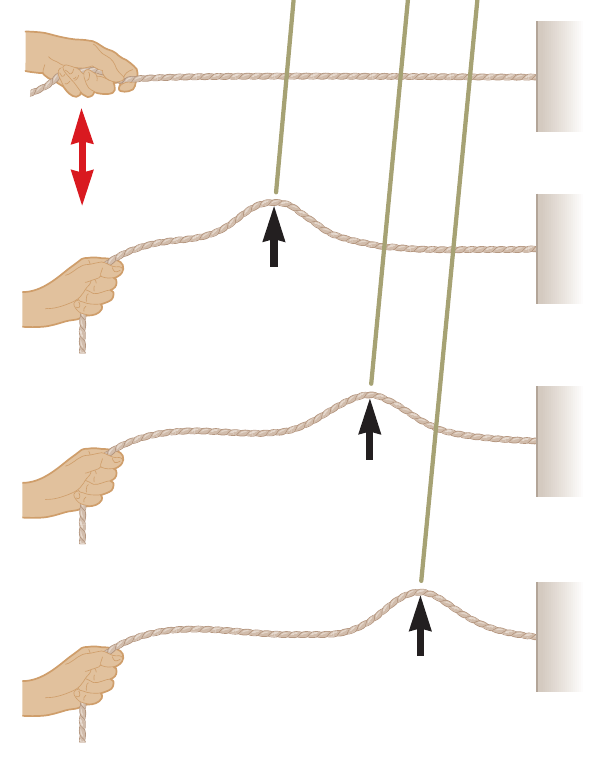
\includegraphics[scale=0.3]{images/oaw/pod01.png}
\end{center}

In this example, the hand is the source of the disturbance, the string is the medium, and the fact 
that the string is connected allows the pulse to travel through the string, disturbing each element 
of the string in the process. Also notice that the pulse has a certain height and speed and the 
shape of the pulse changes very little throughout the whole motion.

\subsection{Types of Disturbance}

Consider a pulse (or wave) traveling along the string. If the elements of the disturbed medium are
moving perpendicular to the direction of propogation, we call said wave a \textbf{transverse wave}.
The pulse on the string example from above is an example of a transverse wave.
In contrast, if the elements of the disturbed medium are moving parallel to the direction of propogation,
we call said wave a \textbf{longitudinal wave}. For example, creating a compressed region on a spring
that moves along it is an example of a longitudinal wave.
\begin{center}
    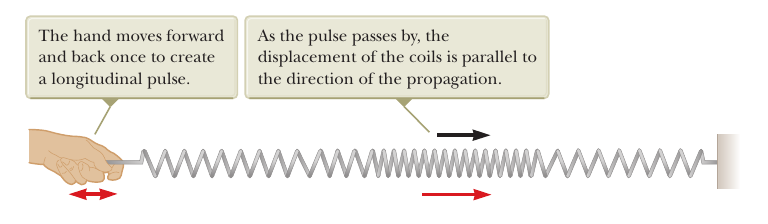
\includegraphics[scale=0.5]{images/oaw/pod02.png}
\end{center}

Some waves in nature are a combination of transverse and longitudinal waves. For example, surface 
water waves actually move in circular path, meaning the disturbance has both transverse and longitudinal
components to it.
\begin{center}
    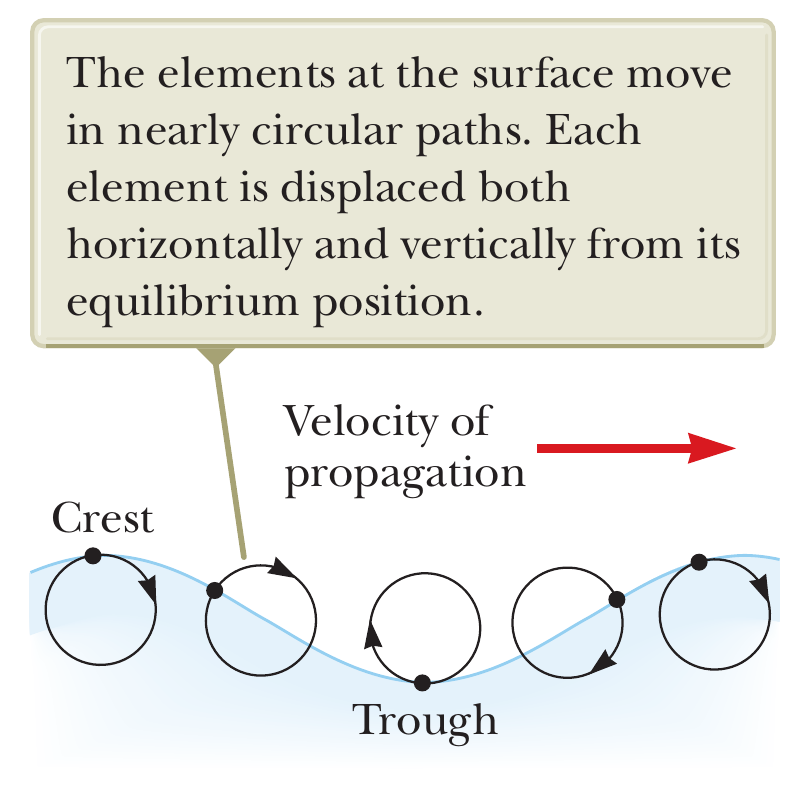
\includegraphics[scale=0.2]{images/oaw/pod03.png}
\end{center}

\subsection{Wave Function}

Consider the following snapshots of a wave propogating.

\begin{figure}[h]
\centering
\begin{subfigure}{0.49\textwidth}
    \centering
    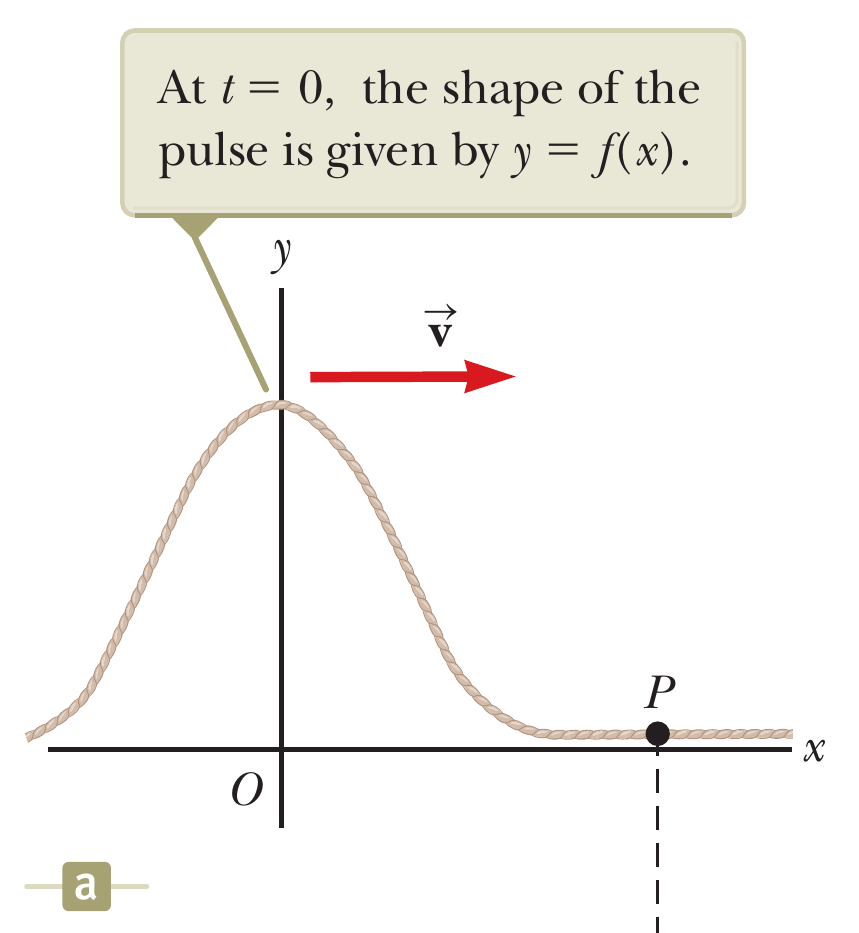
\includegraphics[width=0.9\textwidth]{images/oaw/fig16_5a.png}
\end{subfigure}
% \hfill
\begin{subfigure}{0.49\textwidth}
    \centering
    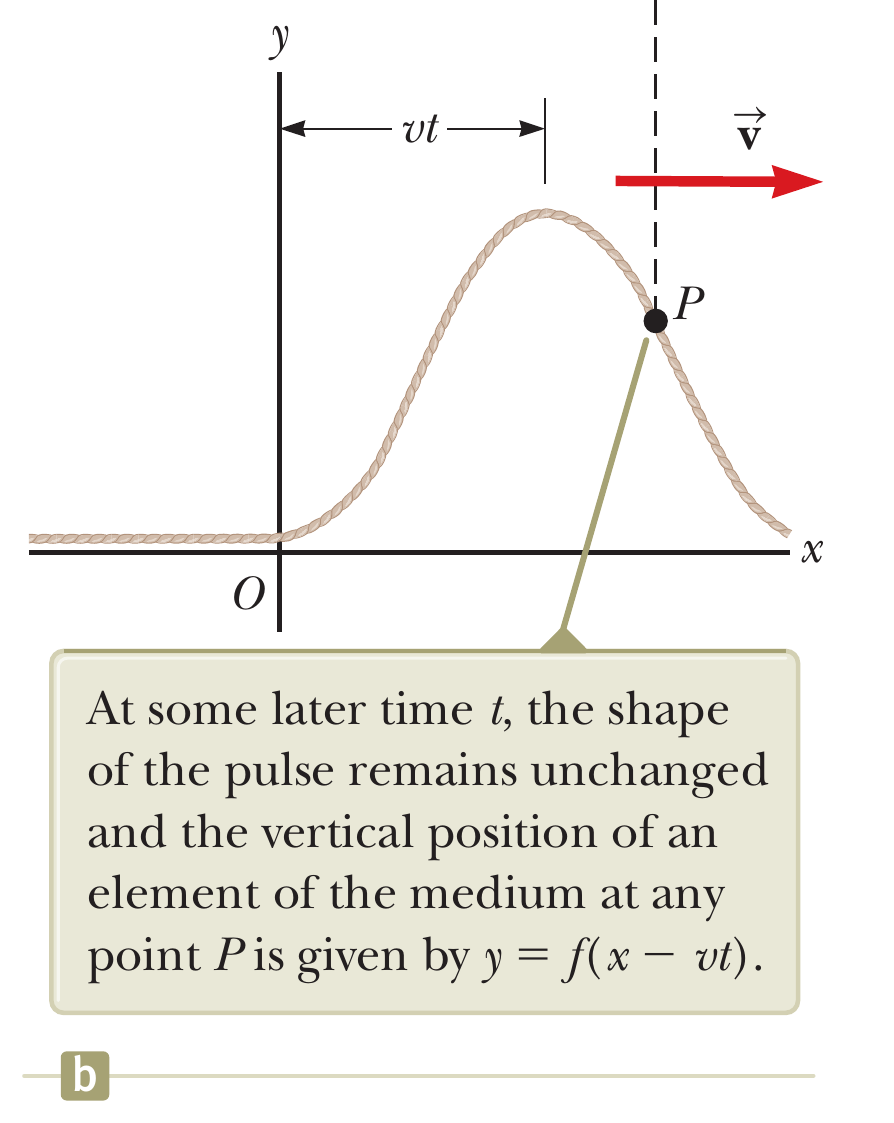
\includegraphics[width=0.9\textwidth]{images/oaw/fig16_5b.png}
\end{subfigure}
\end{figure}

Suppose that the the wave is propogating right with some velocity $\vec{v}$.
Let us represent the shape of the wave with $y(x, t)$. At time $t = 0$, the wave will
have some shape represented by a function $f$, meaning $y(x, 0) = f(x)$ where 
$f$ describes the transverse position $y$ of each element $x$ of the medium at time $t=0$.

Since the pulse moves at speed of $v$, at time $t$, the pulse would have traveled $vt$
to the right at time $t$. Assuming that the shape of the pulse never changes, the shape
of the pulse at time $t$ is the same as when $t=0$. However, $f(x)$ of each $x$ at time
$t$ will have the value of $f(x-vt)$ at time $t=0$, meaning $y(x, t) = y(x-vt, 0)$.

We can express this as the following equation
\begin{equation}\label{16.1}
    y(x, t) = f(x - vt)
\end{equation}
If the pulse were to go left, we simply flip the sign for $vt$.

This function $y(x, t)$ is referred to as the \textbf{wave function}. It represents the 
transverse position at any point $x$ of the medium at time $t$. It also shows at that
at some point $P$, representing a fixed $x$ value, its $y$ will increase, reach its
maximum, the decrease to zero as time goes on.

If $t$ was fixed, function $y(x)$ defines a curve representing the shape of the pulse at
the time. This function $y$ is sometimes called the \textbf{waveform}.

\section{Analysis Model: Traveling Wave}

\cim{images/oaw/sinwave01.png}{0.5}\label{fig16.7}
Here, we will focus on the \textbf{sinusoidal wave} with the shape shown in diagram~\ref{fig16.7}.
Notice that the curve is the same as plotting $\sin\theta$ against $\theta$. It is also known as 
the simplest wave as the medium is disturbed by a single-frequency source.

In a sinusoidal wave, there are two types of motions that can occur:
\begin{itemize}
    \item \textbf{Motion of the wave} refers to the movement of the brown curve where it moves to
        the right until it reaches the blue curve
    \item \textbf{Motion of the elements of the medium} refers to the movement of each element 
        of the medium where $-$ in this case $-$ each element of the medium moves up and down
        in a simple harmonic motion
\end{itemize}

Consider an ideal wave has a single frequency and is infinitely long. We can combine multiple ideal 
waves to build a complex wave, but we will ignore them for now. An ideal wave has the following 
components
\begin{itemize}
    \item \textbf{Crest}: point with highest amplitude
    \item \textbf{Trough}: point with lowest amplitude
    \item \textbf{Wavelength} ($\lambda$): distance between crests, could also refer to the minimum distance
        between two identical points on adjacent waves
    \item \textbf{Period} ($T$): time interval for two identical points in adjacent waves to pass by
        a point
    \item \textbf{Frequency} ($f$): number of times identical points in adjacent waves pass by
        a point in a fixed amount of time, can be computed by $f = 1/T$
        \begin{itemize}
            \item The most common unit for frequency is \textit{hertz} (Hz)
        \end{itemize}
    \item \textbf{Amplitude}: the maximum position an element of the medium relative to its equilibrium poisition
\end{itemize}

Waves travel with a specific speed depneding on the properties of the medium it is traveling through.
For example, the speed at which the sound wave travel through air is diferent than through most solids.

Consider the following snapshots of a sinusoidal wave.

\begin{figure}[h]
\centering
\begin{subfigure}{0.49\textwidth}
    \centering
    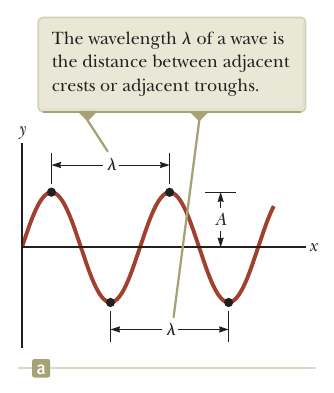
\includegraphics[width=0.9\textwidth]{images/oaw/fig16_8a.png}
\end{subfigure}
\begin{subfigure}{0.49\textwidth}
    \centering
    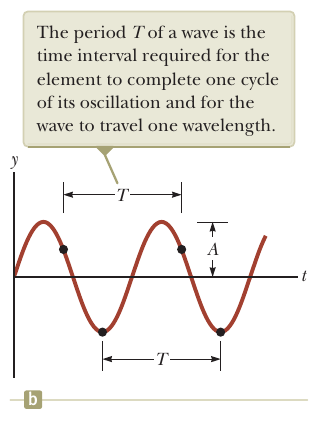
\includegraphics[width=0.9\textwidth]{images/oaw/fig16_8b.png}
\end{subfigure}
\end{figure}

At $t=0$, we can expect the wave function be $y(x, 0) = A\sin(ax)$ where $A$ is the amplitude 
and $a$ is an unknown constant. Notice that $y(0, 0) = A\sin(a\times0) = 0$. Next, notice that 
$y$ is zero again at $x = \lambda/2$. Thus, \[ y\left(\frac{\lambda}{2}, 0\right) =
A\sin\left(a\frac{\lambda}{2}\right) = 0 \]

For this to be true, $a\lambda/2 = \pi$ or $a = 2\pi/\lambda$. Therefore, the function
describing the positions of each element of the sinusoidal wave can be expressed by
\begin{equation}\label{16.4}
    y(x, 0) = A\sin\left(\frac{2\pi}{\lambda}x\right)
\end{equation}

From the diagram, notice that $y$ returns to the same value whenever $x$ is increased by $\lambda$.
Given that the wave is moving to the right at the speed of $v$, we can express the wave function 
at some time $t$, using our discussion on~\eqref{16.1}, as 
\begin{equation}\label{16.5}
    y(x, t) = A\sin\left[\frac{2\pi}{\lambda}(x - vt)\right]
\end{equation}

Using the definition of the different components of a sinusoidal wave, we know that the wave 
travels for $\Delta x = \lambda$ in a time interval $\Delta t = T$. Thus, we can express the speed 
$v$ as 
\begin{equation}\label{16.6}
    v = \frac{\Delta x}{\Delta t} = \frac{\lambda}{T}
\end{equation}

Substituting this $v$ into~\eqref{16.5} will give
\begin{equation}\label{16.7}
    y(x, t) = A\sin\left[2\pi\left(\frac{x}{\lambda} - \frac{t}{T}\right)\right]
\end{equation}
This shows that the wave function is periodic in nature. Also notice that for a fixed $t$, $y$
has the same value at elements $x, x+\lambda, x + 2\lambda, \cdots$. Additionally, for a fixed $x$,
$y$ has the same value at time $t, t+T, t + 2T, \cdots$.

We can further simplify the wave function by defining two more quantities.
\begin{itemize}
    \item \textbf{Angular wave number} (or just wave number) $k$
        \begin{equation}\label{16.8}
            k \equiv \frac{2\pi}{\lambda}
        \end{equation}
    \item \textbf{Angular frequency} $\omega$
        \begin{equation}\label{16.9}
            \omega\equiv \frac{2\pi}{T} = 2\pi f
        \end{equation}
\end{itemize}

If we substitute these into the wave function, we can obtain
\begin{equation}\label{16.10}
    y = A\sin(kx - \omega t)
\end{equation}

Furthermore, we can also substitute them into~\eqref{16.8} and~\eqref{16.9} to get
\begin{eqnarray}
    v = \frac{\omega}{k}\label{16.11}\\
    v = \lambda f\label{16.12}
\end{eqnarray}

Note that the equations above assume that $y(0, 0) = 0$. However, we can introduce a \textit{phase
constant} $\phi$ to shift the waves around so $y(0, 0)$ can be any value. Thus, we can get a general
wave function of
\begin{equation}\label{16.13}
    y(x, t) = A\sin(kx - \omega t + \phi)
\end{equation}
where we can determine the value of $\phi$ ourselves.